\documentclass[preprint, 3p,
authoryear]{elsarticle} %review=doublespace preprint=single 5p=2 column
%%% Begin My package additions %%%%%%%%%%%%%%%%%%%

\usepackage[hyphens]{url}

  \journal{Transport Geography?} % Sets Journal name

\usepackage{graphicx}
%%%%%%%%%%%%%%%% end my additions to header

\usepackage[T1]{fontenc}
\usepackage{lmodern}
\usepackage{amssymb,amsmath}
% TODO: Currently lineno needs to be loaded after amsmath because of conflict
% https://github.com/latex-lineno/lineno/issues/5
\usepackage{lineno} % add
\usepackage{ifxetex,ifluatex}
\usepackage{fixltx2e} % provides \textsubscript
% use upquote if available, for straight quotes in verbatim environments
\IfFileExists{upquote.sty}{\usepackage{upquote}}{}
\ifnum 0\ifxetex 1\fi\ifluatex 1\fi=0 % if pdftex
  \usepackage[utf8]{inputenc}
\else % if luatex or xelatex
  \usepackage{fontspec}
  \ifxetex
    \usepackage{xltxtra,xunicode}
  \fi
  \defaultfontfeatures{Mapping=tex-text,Scale=MatchLowercase}
  \newcommand{\euro}{€}
\fi
% use microtype if available
\IfFileExists{microtype.sty}{\usepackage{microtype}}{}
\usepackage[]{natbib}
\bibliographystyle{plainnat}

\usepackage{graphicx}
\ifxetex
  \usepackage[setpagesize=false, % page size defined by xetex
              unicode=false, % unicode breaks when used with xetex
              xetex]{hyperref}
\else
  \usepackage[unicode=true]{hyperref}
\fi
\hypersetup{breaklinks=true,
            bookmarks=true,
            pdfauthor={},
            pdftitle={Leveraging GTFS to explore spatial gaps in transit supply with respect to social needs},
            colorlinks=false,
            urlcolor=blue,
            linkcolor=magenta,
            pdfborder={0 0 0}}

\setcounter{secnumdepth}{5}
% Pandoc toggle for numbering sections (defaults to be off)


% tightlist command for lists without linebreak
\providecommand{\tightlist}{%
  \setlength{\itemsep}{0pt}\setlength{\parskip}{0pt}}




\usepackage{subfig}
\usepackage{booktabs}
\usepackage{longtable}
\usepackage{array}
\usepackage{multirow}
\usepackage{wrapfig}
\usepackage{float}
\usepackage{colortbl}
\usepackage{pdflscape}
\usepackage{tabu}
\usepackage{threeparttable}
\usepackage{threeparttablex}
\usepackage[normalem]{ulem}
\usepackage{makecell}
\usepackage{xcolor}



\begin{document}


\begin{frontmatter}

  \title{Leveraging GTFS to explore spatial gaps in transit supply with
respect to social needs}
    \author[Public Transport Research Group (PTRG)]{James Reynolds%
  %
  \fnref{1}}
   \ead{james.reynolds@monash.edu} 
    \author[Public Transport Research Group (PTRG)]{Graham Currie%
  \corref{cor1}%
  \fnref{2}}
   \ead{graham.currie@monash.edu} 
    \author[Public Transport Research Group (PTRG)]{Yanda Qu%
  %
  \fnref{3}}
   \ead{yanda.qu@monash.edu} 
      \affiliation[Public Transport Research Group (PTRG)]{
    organization={Public Transport Research Group (PTRG), Institute of
Transport Studies, Department of Civil Engineering Engineering, Monash
University},addressline={Clayton
Campus},city={Melbourne},postcode={3800},state={Victoria},country={Australia},}
    \cortext[cor1]{Corresponding author}
    \fntext[1]{Research Fellow}
    \fntext[2]{Professor}
    \fntext[3]{PhD Student}
  
  \begin{abstract}
  This is the abstract.

  It consists of two paragraphs.
  \end{abstract}
    \begin{keyword}
    keyword1 \sep 
    keyword2
  \end{keyword}
  
 \end{frontmatter}

\section{Introduction}\label{introduction}

A need to provide at least some motorised mobility for those who cannot
otherwise drive themselves influences transit service levels in many
places \citep{Currie:2016aa}. Age, disability, socio-economic status,
lack of a driver's license or vehicle, and many other factors might make
someone reliant on transit services for some or all of their travel.
Social-equity perspectives on transport policy-making, especially the
desire to improve vertical equity so as to better support those who are
disadvantaged (c.f. \citet{Litman:2016aa}), might therefore suggest
providing at least some transit, and probably more than just a minimum,
to places that have the highest social need for transport.

\citet{Currie2003Hobart}, \citet{Currie2004Gap},
\citet{Currie2007Identifying} and \citet{currie2010identifying}
developed an approach for identifying spatial gaps in transit supply
related to social needs for transport. This involves identifying areas
with very high needs for transport, yet little or no service, and was
applied to a case study of 2006 transit service levels in Greater
Melbourne, Australia. However, there does not appear to have been much
further use or development of this approach. As well, it is unclear if
the spatial patterns identified in this previous research, are
representative of transit supply and social needs in other places, or
whether the location of gaps in Melbourne itself have changed in the
intervening years. This may in part be because until recently transit
schedule data was not readily available in consistent, electronic
formats, meaning that assessing transit supply was a large task.

Nowadays, more than 10,000 transit agencies publicly release timetable
data in the General Transit Feed Specification (GTFS) format
\citep{GTFS}. Such standardisation allows Google Maps and other online
platforms to provide outputs for any place with a GTFS feed, and has
facilitated research and other analysis of transit services. However,
tools for using GTFS data to examine spatial patterns and gaps in
transit supply with respect to social needs for transport do not appear
to be readily available. This gap, and the lack of direct follow up to
\citet{Currie2003Hobart}, \citet{Currie2004Gap},
\citet{Currie2007Identifying} and \citet{currie2010identifying}, provide
the motivation for this paper.

The three main objectives of this research are: (1) to develop tools for
undertaking needs-gap analysis using GTFS datasets; (2) to explore
whether such gaps in Melbourne have changed since the publication of
\citet{Currie2007Identifying} and \citet{currie2010identifying}; and (3)
to better understand whether spatial patterns in Melbourne are
representative of those in other places. Research outcomes that are
reported in this paper include the development of a new R package
(gtfssupplyindex) with software tools that facilitate the use of the
\citet{Currie2003Hobart}, \citet{Currie2004Gap},
\citet{Currie2007Identifying} and \citet{currie2010identifying}
approach, in particular the calculation of transit Supply Index (SI)
scores from GTFS datasets. Also presented in this paper are results for
Australian cities in 2016 and 2021, matching the most recent censuses,
which are compared across locations and to the 2006 analysis of
Melbourne reported in \citet{currie2010identifying}.

The remainder of this paper is structured as follows: the next section
outlines the background to this research. Section 3 describes the study
methodology, followed by presentation of results in Section 4 and
discussion in Section 5. Limitations of this study, directions for
future research and a brief conclusion are provided in Section 6.

\section{Research context}\label{research-context}

\subsection{Transit metrics}\label{transit-metrics}

There are many metrics available for benchmarking transit services.
These include those in the Transit Cooperative Research Program (TCRP)
Report 88, a guidebook for developing performance-measurement systems
\citep{Ryus:2003aa}; and those used across benchmarking databases and
programs such as \citet{Florida-Transit-Information-System:2018aa},
\citet{UITP:2015aa} and \citet{Imperial-College-London:2023aa}. The
Fielding Triangle \citep{FieldingGordonJ1987Mpts} provides a framework
for combining indicators of service inputs, outputs and consumption to
describe cost efficiency, cost effectiveness and service effectiveness.
More broadly: \citet{Litman:2003ab} and \citet{Litman:2016aa} discuss
some of the traffic, mobility, accessibility, social equity, strategic
planning and other rational decision-making-based perspectives
underlying many transport indicators; \citet{Reynolds:2017ah} extends
these into models of how institutionalism, incrementalism and other
public policy analysis concepts might apply to decision-making processes
relating to transit prioritization; \citet{GuzmanLuisA.2017Aeit}
developed a measure of accessibility in the context of policy
development and social equity for Latin American Bus Rapid Transit (BRT)
networks; and \citet{Creutzig2020streetspaceallocation} introduced
street space allocation metrics based around ten ethical principles.

However, many of these metrics may be difficult to calculate, explain or
understand, especially for those who are not planners, engineers or
other technical specialists. Where pre-calculated transit metrics are
immediately available, such as on a website or other online platform, it
may not be possible to independently generate scores, for instance to
assess proposed system changes. Contrasting examples are provided by:

\begin{itemize}
\item
  Transit Scores \citep{WalkScore:2023tg}, which are readily available
  online for locations with a published GTFS feed. The meaning of the
  metric appears easy to explain, with the highest possible score of 100
  representing the sort of transit accessibility experienced in the
  center of New York. However, the Transit Score algorithm is secret,
  and scores cannot be calculated independently or generated for
  proposed changes to networks.
\item
  The Transit Capacity and Quality of Service Manual (TCQSM), which
  provides a wide range of metrics for measuring different aspects of a
  transit system. The TCQSM scores themselves appear easy to understand
  or explain, ranging from A (good) to F (bad), although the large
  number of metrics might be somewhat overwhelming for some users. The
  scores, however, can be calculated independently, given sufficient
  data.
\end{itemize}

The widespread availability of GTFS datasets in recent years has
facilitated the development of tools, such as the Transit Score, that
apply the same metric to many transit systems. \citet{Wong:2013aa}
provides an example of what can be done with GTFS data, open metrics and
coding, by reporting the distribution of various TCQSM metrics across 50
USA transit operators. Code used in the \citet{Wong:2013aa} analysis is
available for those who might wish to produce a similar study for other
locations and systems. Developing a similar code base, but for
calculating metrics associated with spatial gaps in transit supply based
on social needs, is the subject of this paper.

\subsection{The Transit Suppy Index}\label{the-transit-suppy-index}

An objective of this study is to produce code that facilitates
calculation of the SI metric from GTFS data. A generalized form of the
SI equation, adapted from \citet{currie2010identifying}, is:

\[SI_{area, time} = \sum{\frac{Area_{Bn}}{Area_{area}}*SL_{n, time}}\]

where:

\begin{itemize}
\item
  \(SI_{area, time}\) is the Supply Index for the area of interest and a
  given period of time;
\item
  \(Area_{Bn}\) is the buffer area for each stop (n) within the area of
  interest (in \citet{currie2010identifying} this was based on a radius
  of 400 metres for bus and tram stops, and 800 metres for railway
  stations);
\item
  \(Area_{area}\) is the area of the area of interest; and
\item
  \(SL_{n,time}\) is the number of transit arrivals for each stop for a
  given time period.
\end{itemize}

\begin{figure}
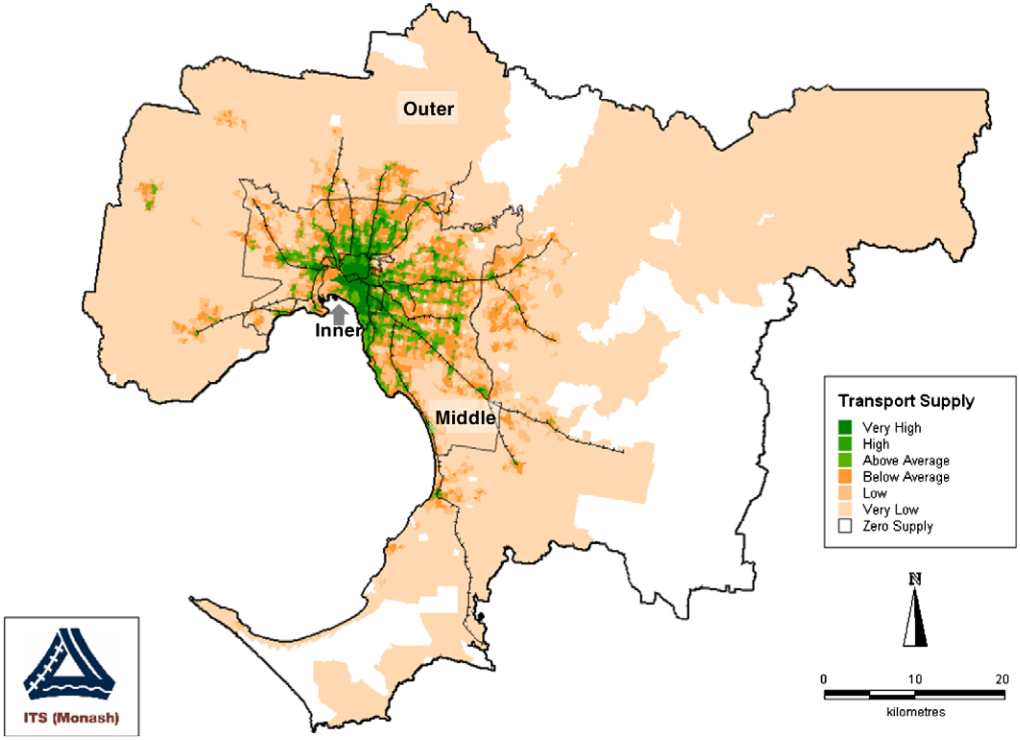
\includegraphics[width=1\linewidth]{graphics/Currie2010SI} \caption{Distribution of supply measure scores – Metropolitan Melbourne (2006), Source: Currie (2010)}\label{fig:Currie_map_SI}
\end{figure}

\citet{currie2010identifying} reported SI scores for Census Collection
Districts (CCDs) across Greater Melbourne in 2006, as shown in Figure
\ref{fig:Currie_map_SI}. General patterns were identified, being: more
transit supply in the middle and inner suburbs, and along passenger
railway lines; and outer areas tending to have very low SI scores or no
transit supply at all.

\subsection{Social need and needs-gap}\label{social-need-and-needs-gap}

As well as measuring transit supply, \citet{currie2010identifying}
assessed the social need for transport across Greater Melbourne using:
the Australian Bureaus of Statistics' Index of Related Socio-Economic
Advantage/Disadvantage (IRSAD) and a transport needs index derived from
eight weighted indicators. The spatial distribution of this composite
social needs index in 2006, reproduced in Figure
\textbackslash ref\{fig:Currie\_map\_needs), showed that areas of above
average, high and very high social needs in 2006 were located in: some
outer areas, particularly in the east and south-east; and in some middle
areas in the south-east, north and west.

\begin{figure}
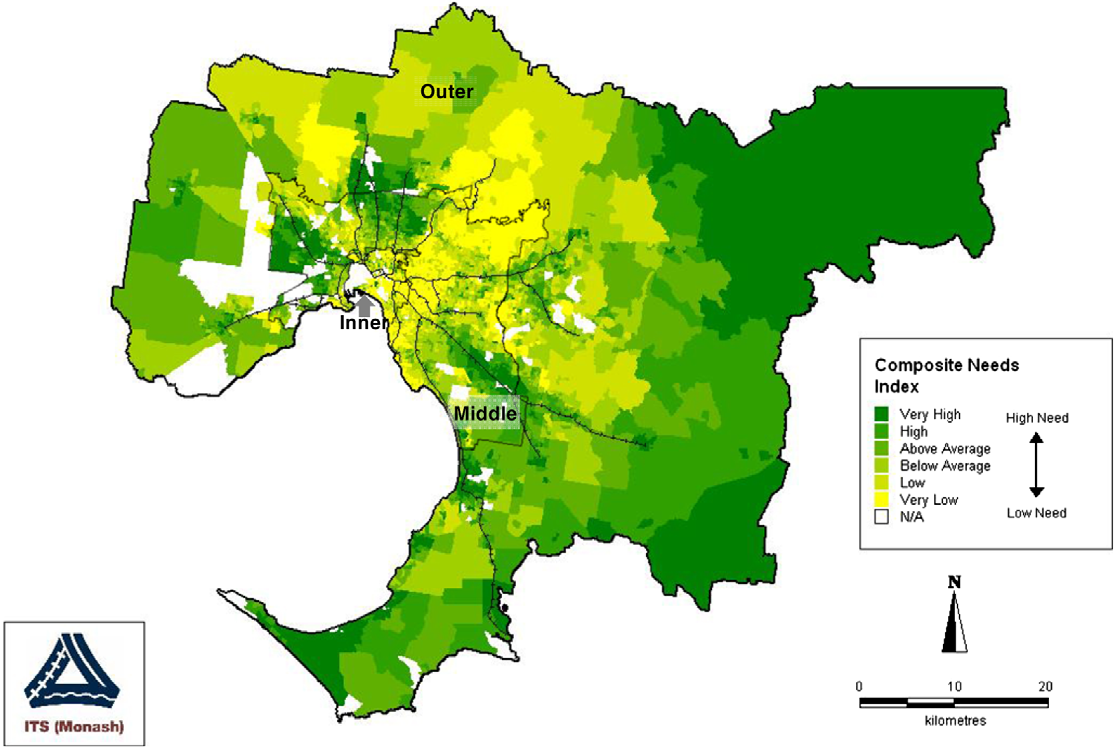
\includegraphics[width=1\linewidth]{graphics/Currie2010Needs} \caption{Distribution of categories of composite social need index scores in 2006. Source: Currie (2010.)}\label{fig:Currie_map_needs}
\end{figure}

As the final step in the spatial needs-gap analysis,
\citet{currie2010identifying} identified areas with very high transport
needs, but very low or no transit supply, as reproduced in Figure
\ref{fig:Currie_map_gap}. These areas were identified as being those
where service gaps might be of particular concern. Most of these were
located in outer parts of Melbourne in the north-east, south-east and
south, although there were also some pockets in the middle suburbs in
the west, north and south east. Overall, \citet{currie2010identifying}
found that ``8.2\% of Melbourne residents have `very high' needs but
`zero', `low' or `very low' public transport supply.''

\begin{figure}
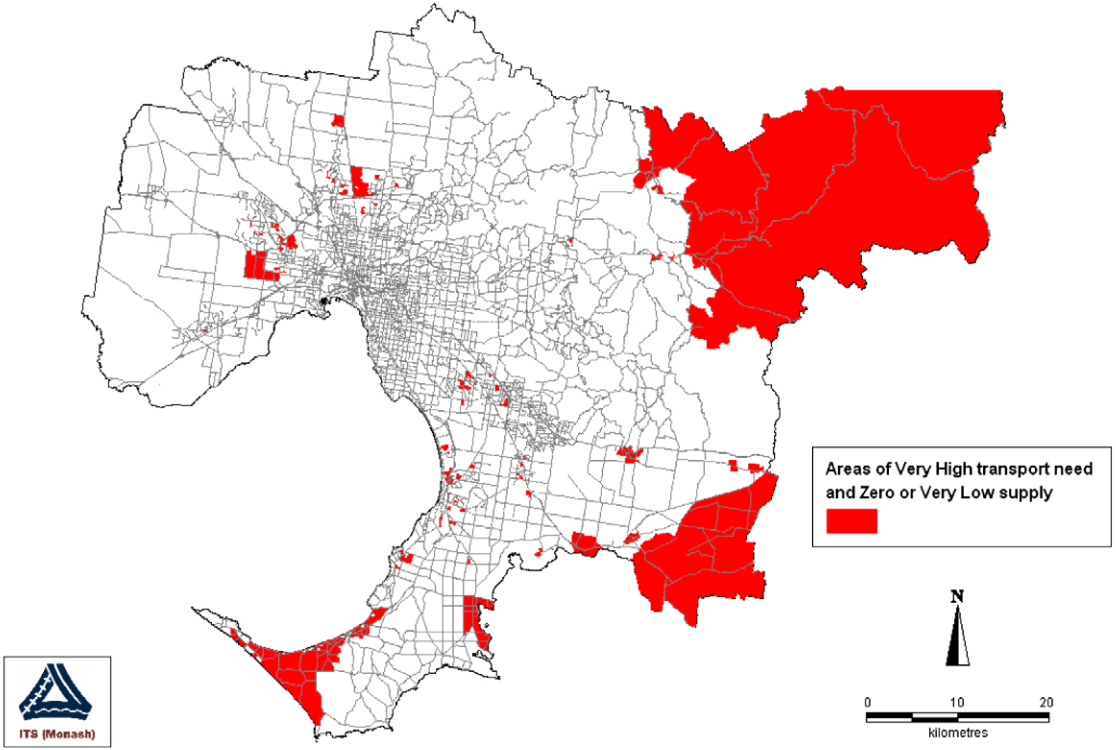
\includegraphics[width=1\linewidth]{graphics/Currie2010gap} \caption{Melbourne needs-gap in 2006 – very high transport need areas with zero or very low public transport supply, Source: Currie (2010)}\label{fig:Currie_map_gap}
\end{figure}

Using this methodology in transit planning was suggested as
``substantially more useful than the presentation of anecdotal evidence,
which is the most common means of identifying transport needs in local
transport studies throughout the world''\citep{currie2010identifying}.
However, it does not appear that this approach has been widely adopted
in practice or by researchers. Our suspicion is that while the SI has a
relatively simple formula and requires only geographic and timetable
data to calculate, a lack of software tools may be partly why it has not
been more widely adopted.

It is also unclear whether the patterns in Melbourne identified in
\citet{currie2010identifying} have changed since the 2006 analysis, or
if Melbourne is representative of other locations. Developing a software
tool to calculate SI tools from GTFS data, and then using it to
comparing current conditions and other locations to the findings of
\citet{currie2010identifying}, therefore, provides the motivation for
this research.

\section{Methodology}\label{methodology}

\subsection{Code development}\label{code-development}

This study developed a package of tools for calculating the SI from GTFS
data using the R programming language \citep{R-base}. The
recommendations of \citet{wickham2023r} informed the package setup and
development approach. Various existing packages and code examples were
relied upon including: the sf package \citep{R-sf} for geospatial
analysis; the tidyverse \citep{tidyverse2019}; gtfstools
\citep{R-gtfstools}; and tidytransit \citep{R-tidytransit}. Australian
Bureau of Statistics (ABS) data was also used, sourced via the strayr
and absmapsdata packages \citep{r-strayr}.

Code was developed and tested on the Mornington Peninsula Tourist
Railway GTFS feed. This was selected primarily for convenience, given
that the authors are familiar with the surrounding geography and that
the feed covers a small number of trips across just three stations.

\subsection{Changes since 2006: Greater
Melbourne}\label{changes-since-2006-greater-melbourne}

Much has changed since 2006, including the spatial geography used by the
Australian Bureau of Statistics (ABS) to collect census data. To allow
direct comparison between 2006 and the most recent census, therefore,
this study calculated SI scores using the same Census Collection
Districts (CCDs) used by \citet{currie2010identifying} for the week
starting the day of the 2021 census. The Victorian GTFS feed, published
by Public Transport Victoria (PTV), was used with historical feeds
sourced via \citet{transitfeeds_victoria:2023aa}.

Unfortunately, it is not possible to obtain 2016 or 2021 social
disadvantage data for CCDs, as the ABS no longer releases data using
this geographic scheme. Population and other statistics are now released
for Statistical Area 1 (SA1) zones. These are updated prior to each
census, typically so as to subdivide zones where populations have
increased. As such, SI scores were also calculated for Greater Melbourne
using the SA1 2021 boundaries, so as to allow a 2021 needs-gap analysis.

\subsection{Variation in spatial patterns across location and
time.}\label{variation-in-spatial-patterns-across-location-and-time.}

SI scores were also calculated for other capital cities in Australia,
for the weeks starting on the days of the 2016 and 2021 censuses.
Historical GTFS data was again sourced via the Transit Feeds website.
Unfortunately it was not possible to locate 2021 GTFS data for Greater
Sydney or Greater Darwin, so SI scores were calculated for 2024 using
the latest data sets, sourced directly from the relevant transit
authorities.

SI scores for 2016 where calculated using both the SA1 2016 and SA1 2021
boundaries. This allowed direct comparisons of SI scores between 2016
and 2021 (using the SA1 2021 boundaries), and comparison of needs-gaps
as 2016 population and social needs data is only released for the SA1
2016 boundaries.

\subsection{Measuring social
disadvantage}\label{measuring-social-disadvantage}

This study adopts a similar approach to measuring social disadvantage as
used in \citet{currie2010identifying}, using: the ABS' Index of Relative
Socio-Economic Advantage/Disadvantage (IRSAD); and a transport needs
index\footnote{The same need indicators and weightings used in
  \citet{currie2010identifying} were adopted, although \$799 or lower
  per week was used as the threshold for low income households rather
  than \$499 to account for inflation (as per the Reserve Bank of
  Australia's online inflation calculator).}. A composite needs
indicator was derived based on the IRSAD and the transport needs index,
again as per the \citet{currie2010identifying} approach. However,
changes to the ABS reporting systems mean that the composite needs
indicator had to be based on weighting both the IRSAD index and the
transport need index by the total population of each SA1 zone, which
were then added, standardised and split into six groups\footnote{This
  contrasts to the method used by \citet{currie2010identifying}, where
  the composite needs index also included relative need components,
  being the IRSAD and the transport needs indexes weighted by the
  population within the various needs groups in each area of interest.}.

\section{Results}\label{results}

\subsection{The gtfssupplyindex
Package}\label{the-gtfssupplyindex-package}

Code developed to calculate SI scores is available as an R package on
github (see \citet{gtfssupplyindex_github}). Included in the package is
a that outlines the structure of the calculations, the developed
functions (LINK HERE), and step-by-step calculations for the Mornington
Peninsula Railway as a worked example. Also included and comparison to
SI scores calculated manually.

\subsection{Greater Melbourne in 2021: changes since
2006}\label{greater-melbourne-in-2021-changes-since-2006}

\subsubsection{SI scores}\label{si-scores}

\begin{figure}
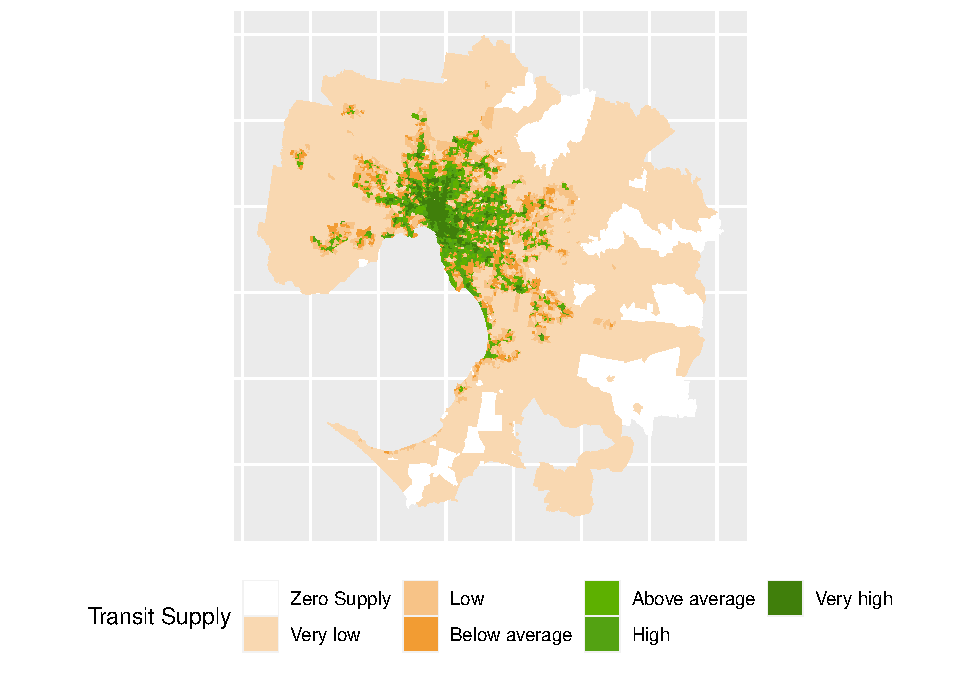
\includegraphics[width=1\linewidth]{Leveraging_GTFS_to_assess_transit_supply_Transport_Geography_files/figure-latex/Greater_Melbourne_CCD_2021-1} \caption{Greater Melbourne (2006 extents), Transport Supply by CCD, week starting the day of the 2021 census}\label{fig:Greater_Melbourne_CCD_2021}
\end{figure}

Figure \ref{fig:Greater_Melbourne_CCD_2021} shows the amount of transit
supply across Greater Melbourne in the week of the 2021 census, using
the same (2006) CCD boundaries as in Figure
\ref{fig:Currie_map_SI}\footnote{The same Transport Supply
  categorizations have been used as in \citet{currie2010identifying},
  with those CCDs that have above average SI scores split evenly into
  three groups, those that have below average SIs also split evenly into
  three groups, and those CCDs without SI scores of zero placed in their
  own category. Hence, both Figure \ref{fig:Currie_map_SI} and Figure
  \ref{fig:Greater_Melbourne_CCD_2021} show relative service levels in
  each CCD compared to the rest of Greater Melbourne for that year.}.
The overall spatial patterns appear generally similar in 2021 as they
were in 2006, with higher levels of transit supply in inner areas and
close to most railway lines. However, there are some clear differences,
including:

\begin{itemize}
\tightlist
\item
  in the south-west (Werribee) service levels and coverage appear to
  have increased.
\item
  the 2021 map shows railway extensions to Sunbury (north-west) and
  Craigieburn (north), both of which involved electrification to
  incorporate existing line segments (already served by country
  services) into the surburban network. Transport Supply to Sunbury,
  however, appears to still be below average, suggesting that not much
  has changed following the shift from service by regional trains to
  suburban trains. For Craigieburn, in contrast, there has been
  increases in service levels, with some areas now having Above Average
  supply.
\item
  in the outer west (Melton) transport supply has fallen below average
\item
  less of the inner area appears to be covered by Very High transport
  supply, although most of this remains Above Average or High, with the
  exception of Albert Park (immediately south of the city centre) which
  has dropped below average;
\item
  some middle south-eastern suburbs along the bay (vicinty of Black
  Roack) have dropped below average;
\item
  Service levels have increased in some parts of the middle north-east
  (Doncaster and Croydon), outer-east (Berwick) and outer south-east
  (Cranbourne).
\item
  Services appear to have been introduced to some outer eastern (east of
  Gembrook), south-eastern (Koo Wee Rup, Lang Lang, Nar Nar Goon,
  Garfield, Bunyip and others) and southern (St Andrews Beach) areas.
\end{itemize}

\begin{table}

\caption{\label{tab:Greater_Melbourne_SA1_2021_table}Greater Melbourne: Distribution of Transport Supply to CCDs (2006, 2021),  SA1s (2021) and resident population (2006, 2021). Sources: 2006 values - Currie (2010), 2021 values - authors analysis}
\centering
\begin{tabular}[t]{l|r|r|r|r|r}
\hline
\multicolumn{1}{c|}{Transport} & \multicolumn{2}{c|}{CCDs} & \multicolumn{1}{c|}{SA1s} & \multicolumn{2}{c}{Population} \\
\cline{1-1} \cline{2-3} \cline{4-4} \cline{5-6}
Supply & 2006 & 2021 & 2021 & 2006 & 2021\\
\hline
Zero Supply & 3.2\%   (189) & 1.3\%    (81) & 4.3\%    (489) & 2.5\%    (85,423) & 3.8\%   (186,829)\\
\hline
Very Low & 22.5\% (1,314) & 23.3\% (1,474) & 23.4\%  (2,692) & 23.6\%   (793,046) & 23.0\% (1,132,967)\\
\hline
Low & 22.4\% (1,310) & 23.3\% (1,473) & 23.4\%  (2,691) & 25.7\%   (865,330) & 23.7\% (1,163,358)\\
\hline
Below average & 22.2\% (1,294) & 23.3\% (1,474) & 23.4\%  (2,691) & 23.0\%   (774,521) & 23.6\% (1,159,783)\\
\hline
Above average & 10.4\%   (608) & 9.6\%   (608) & 8.5\%    (975) & 9.6\%   (324,546) & 8.7\%   (426,892)\\
\hline
High & 9.2\%   (535) & 9.6\%   (608) & 8.5\%    (974) & 7.7\%   (260,411) & 8.7\%   (425,779)\\
\hline
Very High & 10.1\%   (589) & 9.6\%   (608) & 8.5\%    (975) & 7.8\%   (263,832) & 8.6\%   (422,025)\\
\hline
Total & 100.0\% (5,839) & 100.0\% (6,326) & 100.0\% (11,487) & 100.0\% (3,367,109) & 100.0\% (4,917,633)\\
\hline
\end{tabular}
\end{table}

Table \ref{tab:Greater_Melbourne_SA1_2021_table} summarises the
distribution of CCDs, SA1s and resident population across different
Transport Supply categories in 2006 and 2021. The differences between
the share of CCDs in each category in 2006 and 2021 are statistically
significant (\(\chi^2(6, N = 12165) = 59.20\), \(p < .001\)), with only
81 in 2021 (1.3\%) of CCDs in Greater Melbourne (2006 boundary) having
Zero Supply in 2021, compared to the 189 of the 5,839 (3.2\%) reported
by \citet{currie2010identifying} reporting for 2006\footnote{Note,
  however, that there are some inconsistencies in the number of CCDs for
  Melbourne as a whole reported in \citet{currie2010identifying} (5,839)
  and the number included in ABS dataset used for this analysis. This
  appears to be in part related to the inclusion of areas around Western
  Port (south-east), as shown in Figure
  \ref{fig:Greater_Melbourne_CCD_2021}, despite these appearing to be
  outside the 2006 Melbourne boundary.}. However, Greater Melbourne is
now larger than it was in 2006, and the 2021 statistical boundary
includes some additional areas to the north. As such, Table
\ref{tab:Greater_Melbourne_SA1_2021_table} also shows the distribution
of SA1s to the various supply categories, adopting the 2021 SA1 zones
and boundary of Greater Melbourne. Again, the differences between 2006
(CCDs) and 2021 (SA1s) are statistically significant
(\(\chi^2(6, N = 17326) = 44.83\), \(p < .001\)), but there are a
greater proportion with Zero Supply in 2021 (4.3\%) than in 2006. The
share of SA1s with supply below the average (i.e.~Zero, Very Low, Low or
Below Average) is also larger in 2021 (74.5\% versus only 70.3\% in
2006).

Table \ref{tab:Greater_Melbourne_SA1_2021_table} also indicates that
more of the population of Greater Melbourne are within areas with Zero
Supply in 2021 (3.8\%, 186,829 residents) than in 2006 (2.5\%, 85,423
residents), with differences again being statistically significant
(\(\chi^2(6, N = 8284742) = 19038.97\), \(p < .001\)). However, the
share of people living in areas with supply that is below the average
has decreased from 74.8\% to 74.1\%(\(\chi^2(1, N = 8284742) = 532.56\),
\(p < .001\), \(\phi = .01\))

The average SI value has also increased to 3,389.5 in from the value of
2,886.9 in 2006 reported in \citet{currie2010identifying}, indicating
that the overall transit service supply score has increased by
approximately 31\%. SI scores average 12,275.7, 3,409.1 and 998.6 for
the inner, middle and outer suburbs respectively\footnote{The same
  grouping of LGAs to inner, middle and outer suburb groups as used in
  \citet{currie2010identifying} was used for this analysis, although
  here the City of Stonnington was allocated entirely to the middle
  grouping, whereas \citet{currie2010identifying} allocated part of this
  LGA to the inner group.}, compared to 10,922.7, 2,694.9 and 764.3,
respectively, reported for 2006 in \citet{currie2010identifying}.

\subsubsection{Social needs}\label{social-needs}

Figure \ref{fig:Greater_Melbourne_2021_social_needs} shows the
distribution of categories of social need index scores across Greater
Melbourne for 2021. This figure is analogous to the 2006 value from
\citet{currie2010identifying} shown in Figure \ref{fig:Currie_map_needs}
although, as discussed in the methodology section above, it was not
possible to exactly replicate the \citet{currie2010identifying} approach
due to changes in the way census results are reported.

\begin{figure}
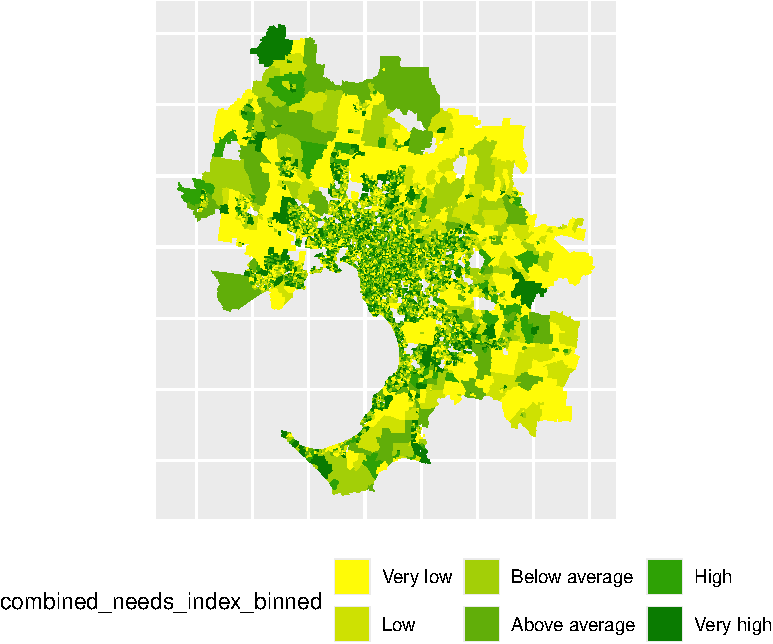
\includegraphics[width=0.9\linewidth]{Leveraging_GTFS_to_assess_transit_supply_Transport_Geography_files/figure-latex/Greater_Melbourne_2021_social_needs-1} \caption{Distribution of categories of composite social need index scores, overlayed with: 2006 Greater Melbourne boundary (black); middle/outer and inner/middle suburb boundaries (grey); and suburban railway lines (dashed).}\label{fig:Greater_Melbourne_2021_social_needs}
\end{figure}

Comparing Figure \ref{fig:Greater_Melbourne_2021_social_needs} and
Figure \ref{fig:Currie_map_needs} suggests that in 2021, compared to
2006: the spatial grouping of different levels of social need is less
consistent; middle eastern suburbs have higher relative needs; and outer
suburbs, particularly in the north-east and south-east, have lower
relative needs. However, this may be an artifact of: the differences in
the composite needs scores used in this analysis (due to the lack of
data to assess relative needs) compared to the
\citet{currie2010identifying} analysis; and the shift of the ABS from
using CCDs to SA1s\footnote{CCDs were originally devised to group the
  approximately 200 dwellings allocated to each individual census
  collector, whereas SA1s were introduced in be consistent in population
  (200 to 800 people, averaging 400) and character\citep{ABS_SA1s_CCDs}}.

\subsubsection{Needs-gap analysis}\label{needs-gap-analysis}

\begin{figure}
\centering
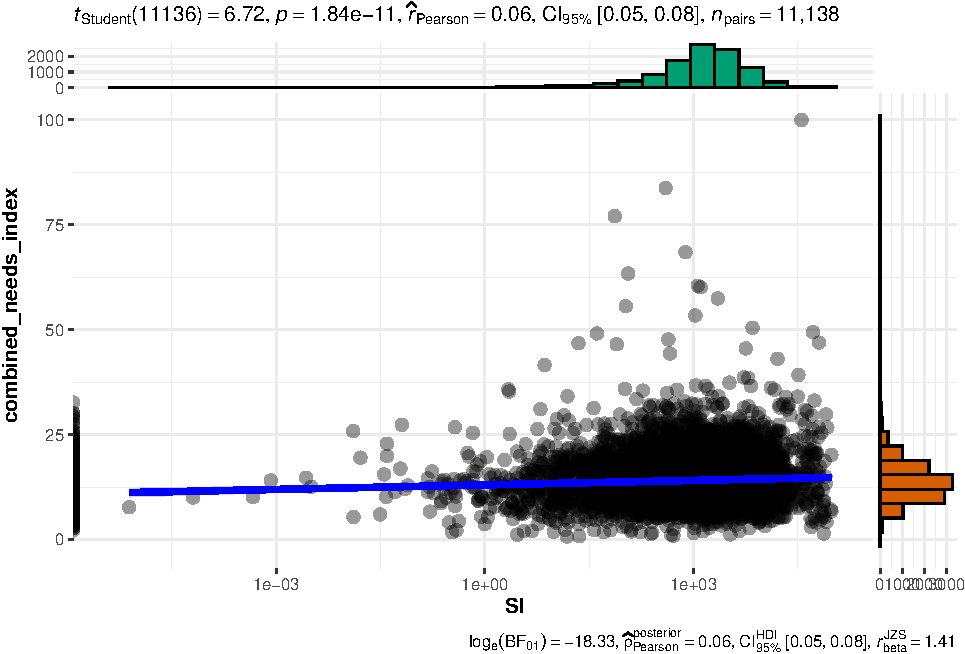
\includegraphics{Leveraging_GTFS_to_assess_transit_supply_Transport_Geography_files/figure-latex/Greater_Melbourne_2021_needs_gap-1.pdf}
\caption{Greater Melbourne 2021, SI and Combined Needs Index scores,
with SI scores \textless{} 1 rounded up to equal 1.}
\end{figure}

Figure \ref{fig:Greater_Melbourne_2021_needs_gap} compares SI and
Combined Needs Index scores for SA1s in 2021. There is a significant,
but only weakly positive relationship.

\begin{table}

\caption{\label{tab:Greater_Melbourne_2021_needs_gap_zones}Greater Melbourne 2021, SA1s within each SI and Combined Needs Index grouping}
\centering
\fontsize{7}{9}\selectfont
\begin{tabular}[t]{l|r|r|r|r|r|r|r}
\hline
transit\_supply & Very Low & Low & Below average & Above average & High & Very High & Total\\
\hline
Zero Supply & 6.4\%   (130) & 4.7\%    (95) & 3.9\%    (79) & 2.9\%    (49) & 3.0\%    (51) & 3.6\%    (61) & 4.2\%    (465)\\
\hline
Very Low & 25.6\%   (520) & 22.3\%   (454) & 21.7\%   (442) & 21.0\%   (353) & 22.0\%   (369) & 24.3\%   (408) & 22.9\%  (2,546)\\
\hline
Low & 23.5\%   (478) & 25.3\%   (514) & 24.6\%   (500) & 24.1\%   (404) & 22.4\%   (376) & 20.6\%   (346) & 23.5\%  (2,618)\\
\hline
Below average & 23.7\%   (483) & 23.6\%   (481) & 23.9\%   (487) & 25.6\%   (430) & 24.6\%   (413) & 20.8\%   (350) & 23.7\%  (2,644)\\
\hline
Above average & 6.9\%   (140) & 8.1\%   (165) & 9.2\%   (188) & 9.3\%   (156) & 9.1\%   (152) & 9.2\%   (155) & 8.6\%    (956)\\
\hline
High & 5.9\%   (120) & 7.9\%   (161) & 9.5\%   (194) & 9.2\%   (154) & 9.7\%   (162) & 9.8\%   (165) & 8.6\%    (956)\\
\hline
Very High & 8.0\%   (163) & 8.1\%   (164) & 7.1\%   (144) & 7.9\%   (133) & 9.2\%   (155) & 11.6\%   (194) & 8.6\%    (953)\\
\hline
Total & 100.0\% (2,034) & 100.0\% (2,034) & 100.0\% (2,034) & 100.0\% (1,679) & 100.0\% (1,678) & 100.0\% (1,679) & 100.0\% (11,138)\\
\hline
\end{tabular}
\end{table}

\begin{figure}
\centering
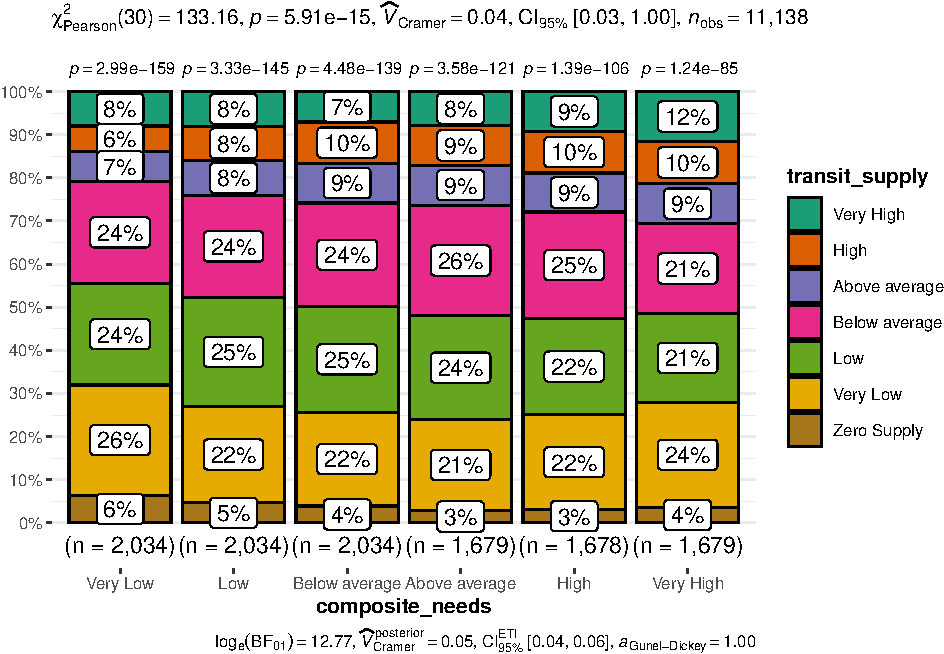
\includegraphics{Leveraging_GTFS_to_assess_transit_supply_Transport_Geography_files/figure-latex/Greater_Melbourne_2021_needs_gap_zones-1.pdf}
\caption{Greater Melbourne 2021, SA1s within each SI and Combined Needs
Index grouping}
\end{figure}

Figure \ref{fig:Greater_Melbourne_2021_needs_gap_zones} and Table
\ref{tab:Greater_Melbourne_2021_needs_gap_zones} compares the SI and
Combined Needs Index groupings for 2021. There is a statistically
significant relationship, although this appears to be weak. 469 SA1s
have zero or very low transit supply, but very high social needs. This
represents 4.2\% of the 11,138 SA1s within Greater Melbourne, and is a
higher proportion than that reported for 2006 (85 of 5,720 CCDs
(1.6\%)).

\begin{table}

\caption{\label{tab:Greater_Melbourne_2021_needs_gap_population}Greater Melbourne 2021, Population in each SI and Combined Needs Index grouping}
\centering
\fontsize{7}{9}\selectfont
\begin{tabular}[t]{l|r|r|r|r|r|r|r}
\hline
transit\_supply & Very Low & Low & Below average & Above average & High & Very High & Total\\
\hline
Zero Supply & 5.7\%  (30,002) & 4.6\%  (32,645) & 3.9\%  (32,328) & 2.9\%  (22,705) & 3.0\%  (27,179) & 3.7\%    (41,915) & 3.8\%   (186,774)\\
\hline
Very Low & 24.4\% (129,294) & 22.4\% (158,919) & 21.7\% (181,719) & 21.1\% (166,490) & 22.3\% (199,467) & 25.6\%   (291,972) & 23.0\% (1,127,861)\\
\hline
Low & 24.6\% (130,477) & 25.8\% (183,274) & 25.1\% (210,538) & 24.5\% (193,642) & 22.9\% (205,397) & 21.0\%   (239,267) & 23.7\% (1,162,595)\\
\hline
Below average & 24.6\% (130,322) & 24.1\% (171,561) & 24.2\% (203,230) & 25.8\% (203,985) & 24.5\% (219,755) & 20.1\%   (229,221) & 23.6\% (1,158,074)\\
\hline
Above average & 7.1\%  (37,419) & 8.0\%  (56,902) & 9.1\%  (76,179) & 9.3\%  (73,062) & 9.0\%  (80,380) & 8.9\%   (100,957) & 8.7\%   (424,899)\\
\hline
High & 6.1\%  (32,274) & 7.6\%  (54,119) & 9.3\%  (77,767) & 8.9\%  (70,132) & 9.4\%  (83,970) & 9.4\%   (107,121) & 8.7\%   (425,383)\\
\hline
Very High & 7.6\%  (40,417) & 7.5\%  (53,477) & 6.7\%  (56,412) & 7.5\%  (59,356) & 8.9\%  (79,306) & 11.4\%   (129,759) & 8.5\%   (418,727)\\
\hline
Total & 100.0\% (530,205) & 100.0\% (710,897) & 100.0\% (838,173) & 100.0\% (789,372) & 100.0\% (895,454) & 100.0\% (1,140,212) & 100.0\% (4,904,313)\\
\hline
\end{tabular}
\end{table}

\begin{figure}
\centering
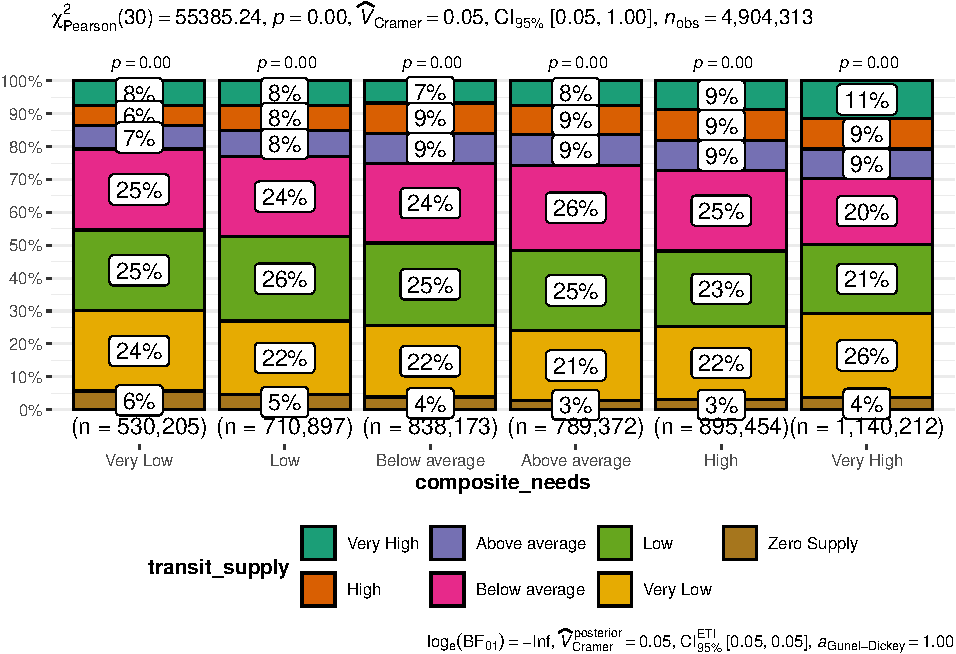
\includegraphics{Leveraging_GTFS_to_assess_transit_supply_Transport_Geography_files/figure-latex/Greater_Melbourne_2021_needs_gap_population-1.pdf}
\caption{Greater Melbourne 2021, Populations within each SI and Combined
Needs Index grouping}
\end{figure}

Figure \ref{fig:Greater_Melbourne_2021_needs_gap_population} and Table
\ref{tab:Greater_Melbourne_2021_needs_gap_population} compares the
populations within each SI and Combined Needs Index grouping for 2021.
There is a statistically significant relationship, although this appears
to be weak. 333887 people live within SA1s that have zero or very low
transit supply, but very high social needs. This represents 6.8\% of the
4,904,313 people within Greater Melbourne, and is a lower proportion
than that reported for 2006 (37,699 of 3.3 million people (8.2\%)).

\begin{figure}
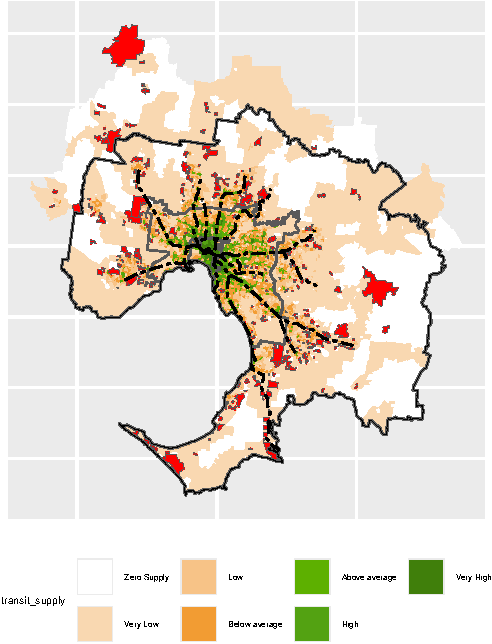
\includegraphics[width=1\linewidth]{Leveraging_GTFS_to_assess_transit_supply_Transport_Geography_files/figure-latex/Greater_Melbourne_2021_needs_gap_map-1} \caption{Greater Melbourne 2021 SI groupings, overlayed with SA1s with very high transport need areas with zero or very low public transport supply (red).}\label{fig:Greater_Melbourne_2021_needs_gap_map}
\end{figure}

Figure \ref{fig:Greater_Melbourne_2021_needs_gap_map} shows SA1 zones in
Greater Melbourne with Very High transport needs, but Very Low or Zero
transit supply for 2021. Comparison to the 2006 spatial distribution
shown in Figrue \ref{fig:Currie_map_gap} suggests that now areas with
social needs gaps are: still mostly in outer suburbs; more widely
distributed across Greater Melbourne; and cover smaller geographical
areas. This last change, however, may again be an artefact of the shift
from CCDs to SA1s, given that SA1s tend to cover smaller areas and be
concentrated on population centres\footnote{For example, Figure
  \ref{fig:Currie_map_gap} shows a large area of very high transport
  need but very low or zero supply in the north-east of Greater
  Melbourne consisting of around 10 CCDs. However, most of this area is
  in the Yarra Ranges National Park or adjoining non-populated areas. In
  contrast, the 2021 map shows only a few small SA1s in the outer
  north-east of Greater Melbourne as having very high social needs but
  very low or zero transit supply (these include SA1s around Heasleville
  and Gembrook), as the SA1 boundaries more closely align to populated
  areas.}

\subsection{Greater Melbourne: 2016 and
2021}\label{greater-melbourne-2016-and-2021}

\subsubsection{SI scores, SA1\_2021
boundaries}\label{si-scores-sa1_2021-boundaries}

\begin{figure}
\centering
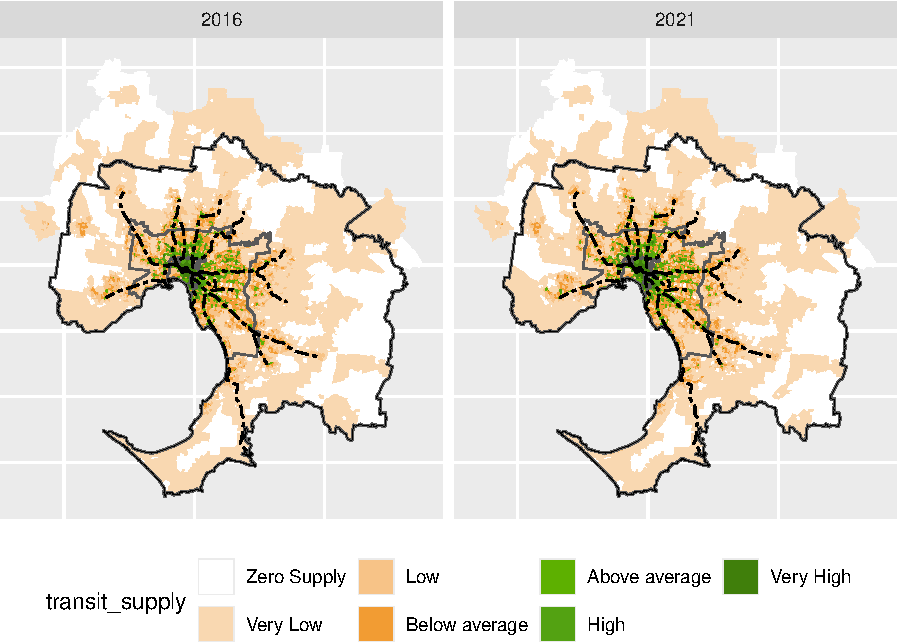
\includegraphics{Leveraging_GTFS_to_assess_transit_supply_Transport_Geography_files/figure-latex/Greater_Melbourne_2016_2021_plot-1.pdf}
\caption{Greater Melbourne, Transit Supply by 2021 SA1 for the weeks
starting the date of 2016 and 2021 census, overlayed with: 2006 Greater
Melbourne boundary (black); middle/outer and inner/middle suburb
boundaries (grey); and suburban railway lines (dashed)}
\end{figure}

\begin{table}

\caption{\label{tab:Greater_Melbourne_SA1_2016_2021_table_and_bar_chart}Greater Melbourne: Distribution of SA1s and resident population to Transit Supply categories, 2016 and 2021, using the 2021 SA1 boundaries}
\centering
\begin{tabular}[t]{l|r|r|r|r}
\hline
\multicolumn{1}{c|}{Transit Supply} & \multicolumn{2}{c|}{2016} & \multicolumn{2}{c}{2021} \\
\cline{1-1} \cline{2-3} \cline{4-5}
category & SA1s & Population & SA1s & Population\\
\hline
Zero Supply & 6.8\%    (780) & 3.6\%   (161,045) & 4.3\%    (489) & 3.8\%   (186,829)\\
\hline
Very Low & 22.9\%  (2,634) & 21.5\%   (966,300) & 23.4\%  (2,692) & 23.0\% (1,132,967)\\
\hline
Low & 22.9\%  (2,633) & 24.2\% (1,083,606) & 23.4\%  (2,691) & 23.7\% (1,163,358)\\
\hline
Below average & 22.9\%  (2,633) & 24.5\% (1,100,603) & 23.4\%  (2,691) & 23.6\% (1,159,783)\\
\hline
Above average & 8.1\%    (936) & 8.8\%   (395,116) & 8.5\%    (975) & 8.7\%   (426,892)\\
\hline
High & 8.1\%    (935) & 8.8\%   (392,868) & 8.5\%    (974) & 8.7\%   (425,779)\\
\hline
Very High & 8.1\%    (936) & 8.6\%   (385,683) & 8.5\%    (975) & 8.6\%   (422,025)\\
\hline
Total & 100.0\% (11,487) & 100.0\% (4,485,221) & 100.0\% (11,487) & 100.0\% (4,917,633)\\
\hline
\end{tabular}
\end{table}

\begin{figure}
\centering
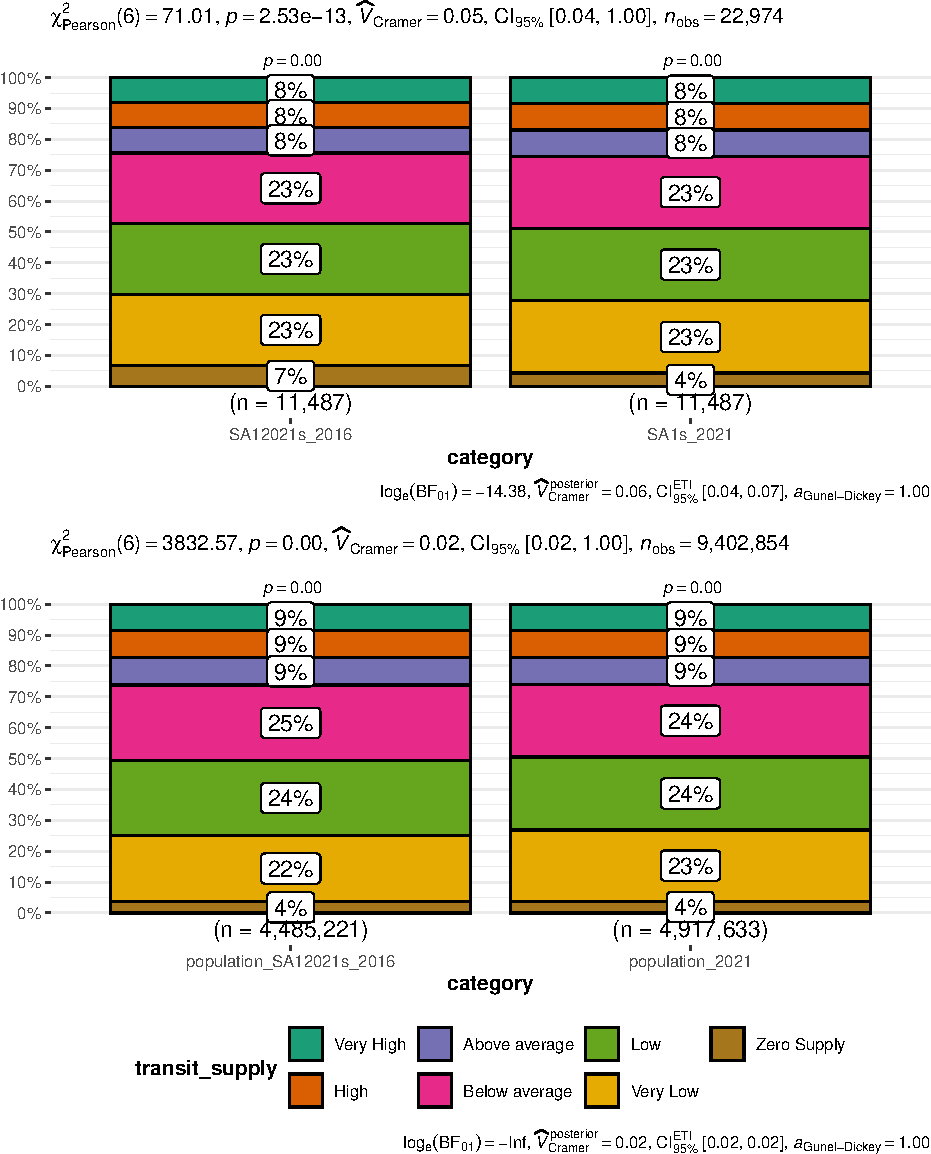
\includegraphics{Leveraging_GTFS_to_assess_transit_supply_Transport_Geography_files/figure-latex/Greater_Melbourne_SA1_2016_2021_table_and_bar_chart-1.pdf}
\caption{Greater Melbourne: distribution of Transit Supply to SA1s (2021
boundaries)(top) and population (bottom) in 2016 and 2021}
\end{figure}

Figure \ref{fig:Greater_Melbourne_2016_2021_plot} maps Transit Supply
for the weeks starting the days of the 2016 and 2021. The spatial
pattern of Transit Supply appears to be largely the same although, as
shown in Table
\ref{tab:Greater_Melbourne_SA1_2016_2021_table_and_bar_chart}, the share
of SA1s with zero transit supply fell from 6.8\% in 2016 to 4.3\% in
2021. Figure
\ref{fig:Greater_Melbourne_SA1_2016_2021_table_and_bar_chart} indicates,
however, that while the differences between 2016 and 2021 in the number
of SA1s and the share of the population in each of the Transit Supply
categories is statistically significant, the changes are small.

\begin{figure}
\centering
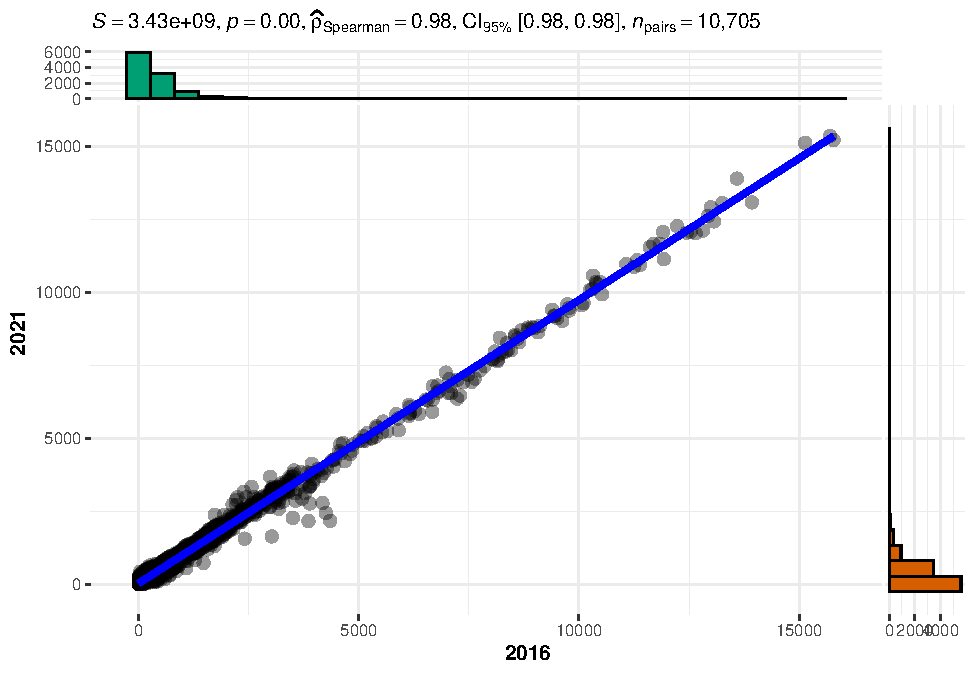
\includegraphics{Leveraging_GTFS_to_assess_transit_supply_Transport_Geography_files/figure-latex/Greater_Melbourne_2016_2021_scatterplot-1.pdf}
\caption{Greater Melbourne: SI scores in 2016 and 2021 by SA1 (2021
boundaries), adjusted to set those \textless1 equal to 1 (for visual
clarity)}
\end{figure}

Figure \ref{fig:Greater_Melbourne_2016_2021_scatterplot} directly
compares the 2016 and 2021 SI scores for each SA1, again using the 2021
SA1 boundaries (note: to reduce the complexity of the graphic, SI scores
less than 1 have been set equal to 1). There is a statistically
significant relationship between the 2016 and 2021 SI scores, and most
SA1s appear to have a similar SI score in both years. However, there are
many SA1s that have higher or lower SI scores in 2021 than in 2016, and
these are summarised in Figure
\ref{fig:Greater_Melbourne_2016_2021_ratio_table} and Table
\ref{tab:Greater_Melbourne_2016_2021_ratio_table}.

\begin{table}

\caption{\label{tab:Greater_Melbourne_2016_2021_ratio_table}Greater Melbourne: changes in SI between 2016 and 2021 by SA1}
\centering
\fontsize{7}{9}\selectfont
\begin{tabular}[t]{>{\raggedright\arraybackslash}p{2cm}|>{\raggedleft\arraybackslash}p{1cm}|>{\raggedleft\arraybackslash}p{1cm}|>{\raggedleft\arraybackslash}p{1cm}|>{\raggedleft\arraybackslash}p{1cm}|>{\raggedleft\arraybackslash}p{1cm}|>{\raggedleft\arraybackslash}p{1cm}|>{\raggedleft\arraybackslash}p{1cm}|>{\raggedleft\arraybackslash}p{1cm}|>{\raggedleft\arraybackslash}p{1cm}|>{\raggedleft\arraybackslash}p{1cm}}
\hline
Change & Inner & Inner East & Inner South & North East & North West & Outer East & South East & West & M'ton P'sula & Total\\
\hline
New service & 0.0\%     (0) & 0.0\%   (0) & 0.0\%   (0) & 1.6\%    (20) & 8.1\%  (79) & 0.1\%     (1) & 5.7\%   (113) & 4.4\%    (87) & 0.8\%   (6) & 2.7\%    (306)\\
\hline
Increased 16\% or more & 2.9\%    (41) & 0.2\%   (2) & 14.0\% (137) & 12.1\%   (155) & 28.1\% (274) & 3.2\%    (41) & 20.0\%   (396) & 20.4\%   (402) & 24.6\% (177) & 14.1\%  (1,625)\\
\hline
Increased 10 to 16\% & 4.7\%    (68) & 0.7\%   (6) & 4.6\%  (45) & 3.7\%    (47) & 3.3\%  (32) & 1.8\%    (23) & 3.5\%    (70) & 6.0\%   (119) & 3.6\%  (26) & 3.8\%    (436)\\
\hline
Increased 4 to 10\% & 16.9\%   (242) & 6.4\%  (56) & 15.3\% (149) & 11.2\%   (144) & 14.6\% (142) & 8.7\%   (111) & 8.2\%   (162) & 17.6\%   (347) & 6.1\%  (44) & 12.2\%  (1,397)\\
\hline
Increased 1 to 4\% & 27.2\%   (390) & 20.9\% (182) & 18.9\% (184) & 23.9\%   (307) & 16.6\% (162) & 9.6\%   (122) & 12.0\%   (238) & 18.7\%   (367) & 12.1\%  (87) & 17.8\%  (2,039)\\
\hline
Increased  less than 1\% & 12.7\%   (183) & 22.2\% (193) & 14.1\% (138) & 14.0\%   (180) & 9.0\%  (88) & 23.4\%   (298) & 14.5\%   (288) & 10.5\%   (206) & 18.3\% (132) & 14.9\%  (1,706)\\
\hline
No change & 0.0\%     (0) & 0.3\%   (3) & 0.3\%   (3) & 0.7\%     (9) & 0.7\%   (7) & 1.8\%    (23) & 1.8\%    (35) & 0.7\%    (14) & 2.8\%  (20) & 1.0\%    (114)\\
\hline
Reduced less than 1\% & 7.2\%   (103) & 28.5\% (248) & 8.4\%  (82) & 8.2\%   (106) & 4.4\%  (43) & 26.7\%   (340) & 15.0\%   (297) & 6.5\%   (127) & 15.1\% (109) & 12.7\%  (1,455)\\
\hline
Reduced by 1 to 10\% & 22.7\%   (326) & 17.8\% (155) & 16.7\% (163) & 15.1\%   (194) & 6.2\%  (60) & 15.2\%   (194) & 6.8\%   (135) & 6.3\%   (123) & 7.9\%  (57) & 12.2\%  (1,407)\\
\hline
Reduced by more than 10\% & 5.8\%    (83) & 2.8\%  (24) & 7.2\%  (70) & 4.0\%    (52) & 3.4\%  (33) & 6.0\%    (77) & 5.4\%   (108) & 3.2\%    (63) & 0.4\%   (3) & 4.5\%    (513)\\
\hline
Service withdrawn & 0.0\%     (0) & 0.0\%   (0) & 0.0\%   (0) & 0.3\%     (4) & 0.1\%   (1) & 0.2\%     (3) & 0.2\%     (3) & 0.2\%     (4) & 0.0\%   (0) & 0.1\%     (15)\\
\hline
Never served & 0.0\%     (0) & 0.1\%   (1) & 0.5\%   (5) & 5.2\%    (67) & 5.5\%  (54) & 3.2\%    (41) & 7.0\%   (139) & 5.5\%   (108) & 8.2\%  (59) & 4.1\%    (474)\\
\hline
Total & 100.0\% (1,436) & 100.0\% (870) & 100.0\% (976) & 100.0\% (1,285) & 100.0\% (975) & 100.0\% (1,274) & 100.0\% (1,984) & 100.0\% (1,967) & 100.0\% (720) & 100.0\% (11,487)\\
\hline
\end{tabular}
\end{table}

\begin{figure}
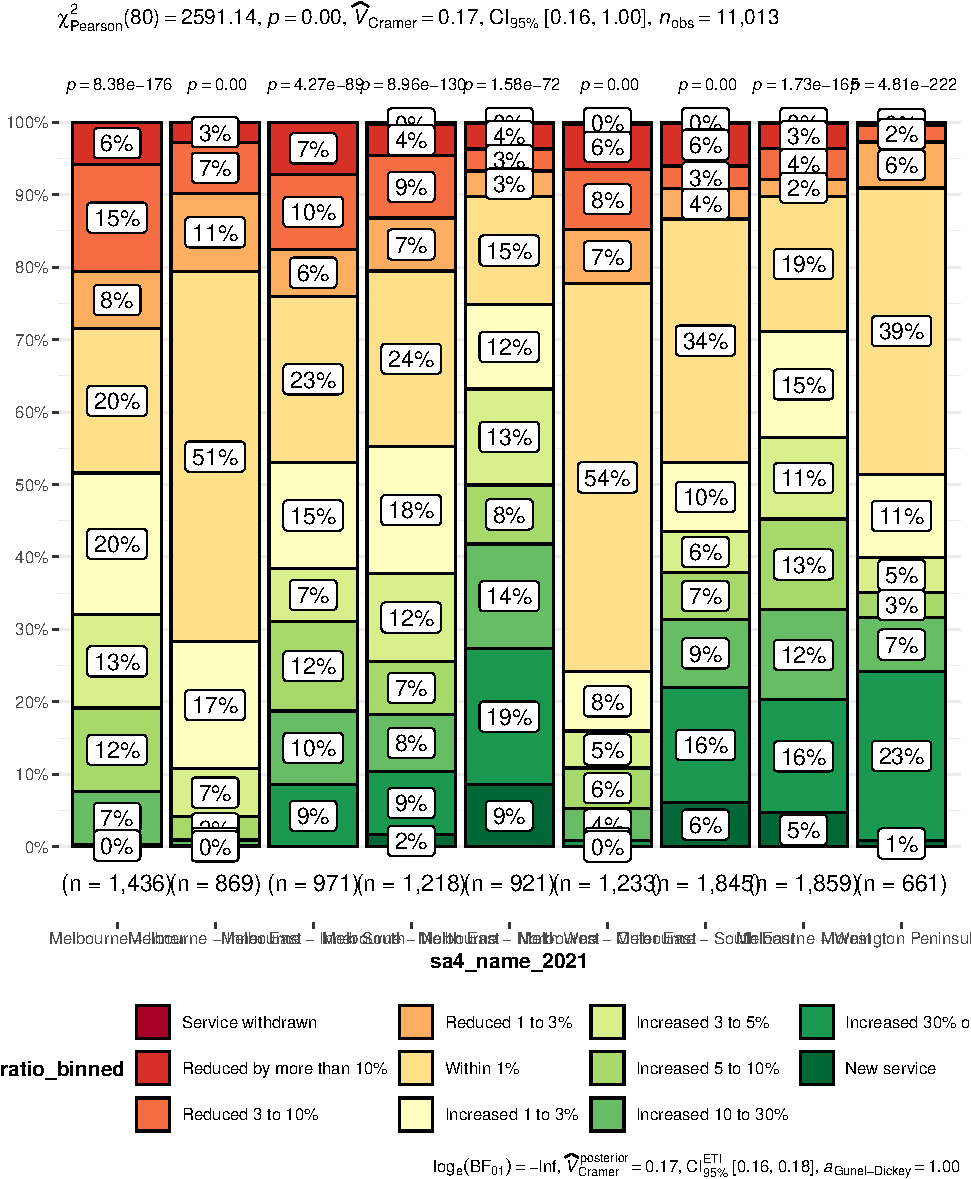
\includegraphics[width=0.9\linewidth]{Leveraging_GTFS_to_assess_transit_supply_Transport_Geography_files/figure-latex/Greater_Melbourne_2016_2021_ratio_table-1} \caption{Greater Melbourne: changes in SI between 2016 and 2021, number of SA1s by SA4}\label{fig:Greater_Melbourne_2016_2021_ratio_table}
\end{figure}

Transit service has been withdrawn entirely between 2016 and 2021 for
15(0.1\%) SA1s, while 513(4.5\%) had SI scores falling by more than 10
percent. At the other end, 2,061(17.9\%) had SI scores increase by 10
percent or more, and 306(2.7\%) SA1s that had no transit in 2016
received at least some service in 2021.

Figure \ref{fig:Greater_Melbourne_2016_2021_ratio_table} compares the
share of SA1s with service level changes in 2021 across SA4 areas. There
is a statistically significant difference across the different spatial
areas of Greater Melbourne, with more SA1s having increased service in
the outer north west and outer west. The inner east and outer east had a
larger share of SA1s with lower levels of transit service.

\begin{figure}
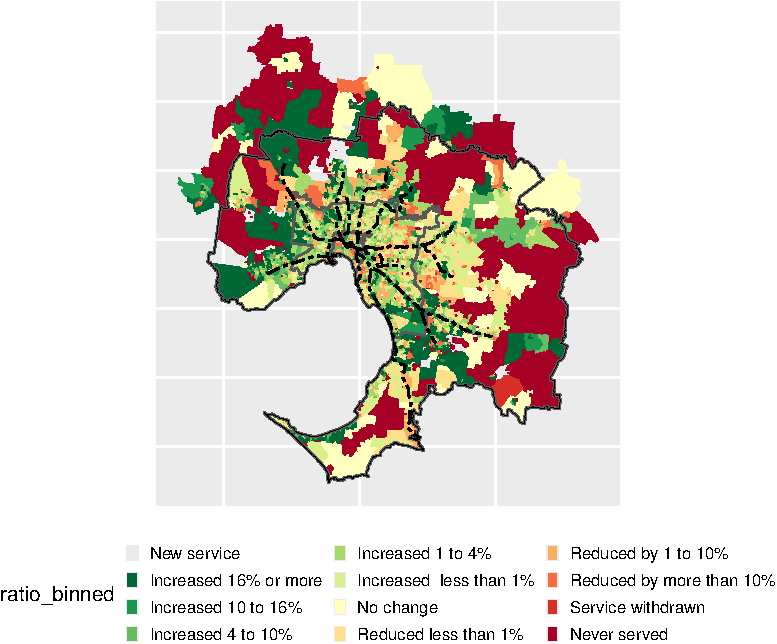
\includegraphics[width=0.9\linewidth]{Leveraging_GTFS_to_assess_transit_supply_Transport_Geography_files/figure-latex/Greater_Melbourne_2016_2021_ratio_map-1} \caption{Greater Melbourne: changes in SI between 2016 and 2021, by SA1}\label{fig:Greater_Melbourne_2016_2021_ratio_map}
\end{figure}

Figure \ref{fig:Greater_Melbourne_2016_2021_ratio_map} maps the changes
in transit service levels. As well as the changes discussed above, the
map suggests other areas that have seen increases, including: around the
Dandenong, Cranbourne, Nar Nar Goon, Garfield and Bunyip areas (outer
south-east); some parts of the Mornington Penninsula; Kinglake (outer
north-east); and around Wallan (outer north). Decreased service levels,
in contrast are also evident: along the Stoney Point Line and Koo Wee
Rup (outer south-east); Heathcote Junction (north of Wallan); and
Diggers Rest (outer north-west).

\subsubsection{SI scores, SA1\_2016
boundaries}\label{si-scores-sa1_2016-boundaries}

Figure \ref{fig:Greater_Melbourne_2016_plot_SA12016} compares the
Transit Supply categories for SA12016 boundaries (left) and 2021
boundaries (right). The spatial patterns appear to be largely similar,
reflecting that there do not appear to have been large changes in the
SA1 boundaries.

\begin{figure}
\centering
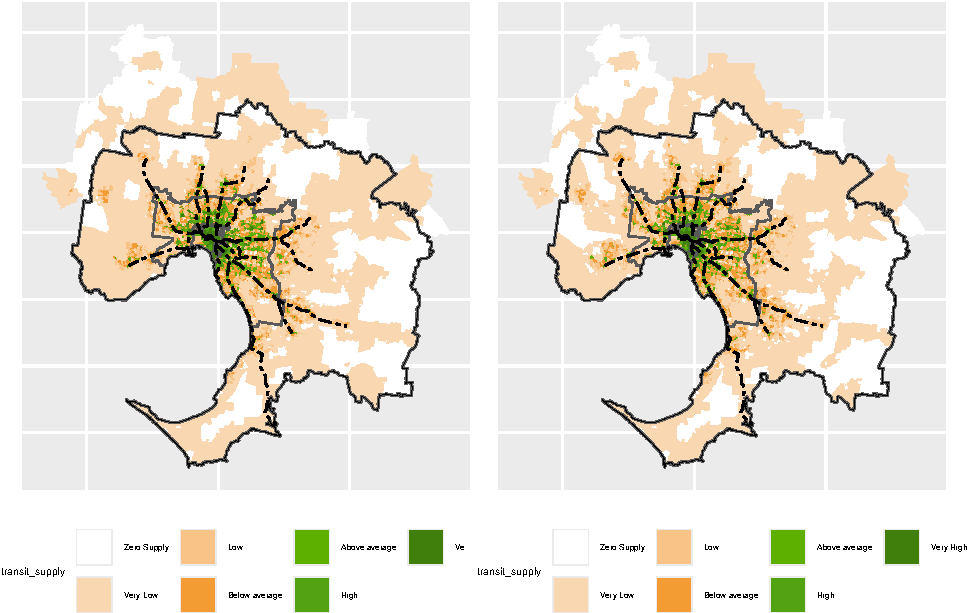
\includegraphics{Leveraging_GTFS_to_assess_transit_supply_Transport_Geography_files/figure-latex/Greater_Melbourne_2016_plot_SA12016-1.pdf}
\caption{Greater Melbourne, Transit Supply by 2016 SA1 for the weeks
starting the date of 2016, overlayed with: 2006 Greater Melbourne
boundary (black); middle/outer and inner/middle suburb boundaries
(grey); and suburban railway lines (dashed)}
\end{figure}

\subsubsection{Social needs}\label{social-needs-1}

\begin{figure}
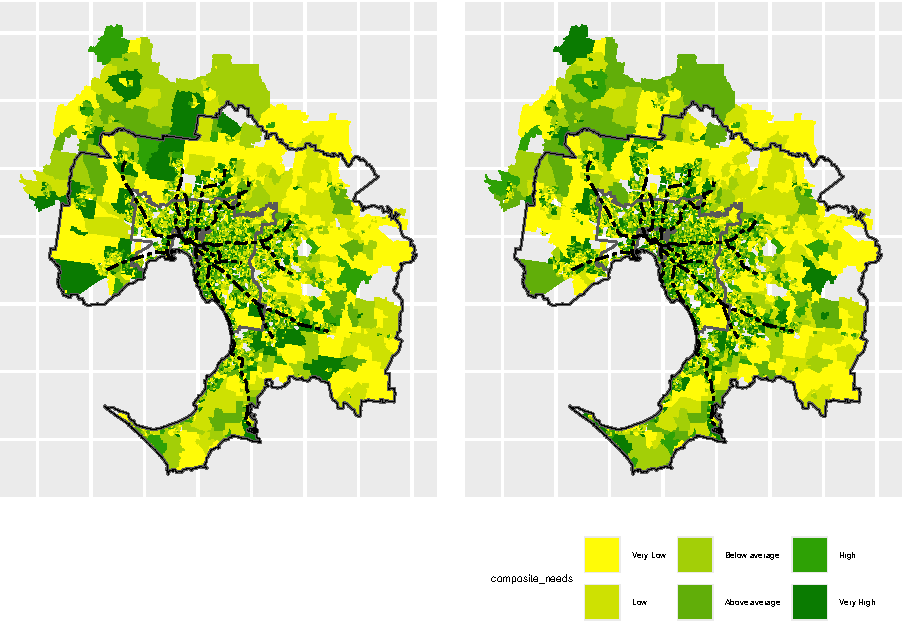
\includegraphics[width=0.9\linewidth]{Leveraging_GTFS_to_assess_transit_supply_Transport_Geography_files/figure-latex/Greater_Melbourne_2016_social_needs-1} \caption{Distribution of categories of composite social need index scores in 2016 (left) and 2021 (right), overlayed with: 2006 Greater Melbourne boundary (black); middle/outer and inner/middle suburb boundaries (grey); and suburban railway lines (dashed).}\label{fig:Greater_Melbourne_2016_social_needs}
\end{figure}

Comparing the 2016 and 2021 maps shown in Figure
\ref{fig:Greater_Melbourne_2016_social_needs} suggests that overall
spatial patterns of social need were generally similar in both years.
Obvious differences include:

\begin{itemize}
\item
  social needs in the southern parts of Bacchus Marsh and areas around
  Melton (outer west) shifted from the Very High category to lower
  categories;
\item
  social needs in some outer northern areas, to the west of Craigieburn
  and north to the area around Wallan also shifted down from the Very
  High category.
\item
  social needs in some outer south-eastern areas, around Dandenong,
  Pakenham, Cranbourne and Koo Wee Rup; and close to end of the
  Mornington Penninsula (south) also shifted down from the Very High
  category.
\end{itemize}

However, it may be that some of these changes are an artefact of changes
to statistical boundaries, with many of these areas appearing to have
been subdivided between 2016 and 2021. Changes in outer areas of Greater
Melbourne also appear to be more obvious, due to the larger size of the
Statistical Area 1 zones in outer parts (due to lower population
density).

\subsubsection{Needs-gap analysis}\label{needs-gap-analysis-1}

\begin{figure}
\centering
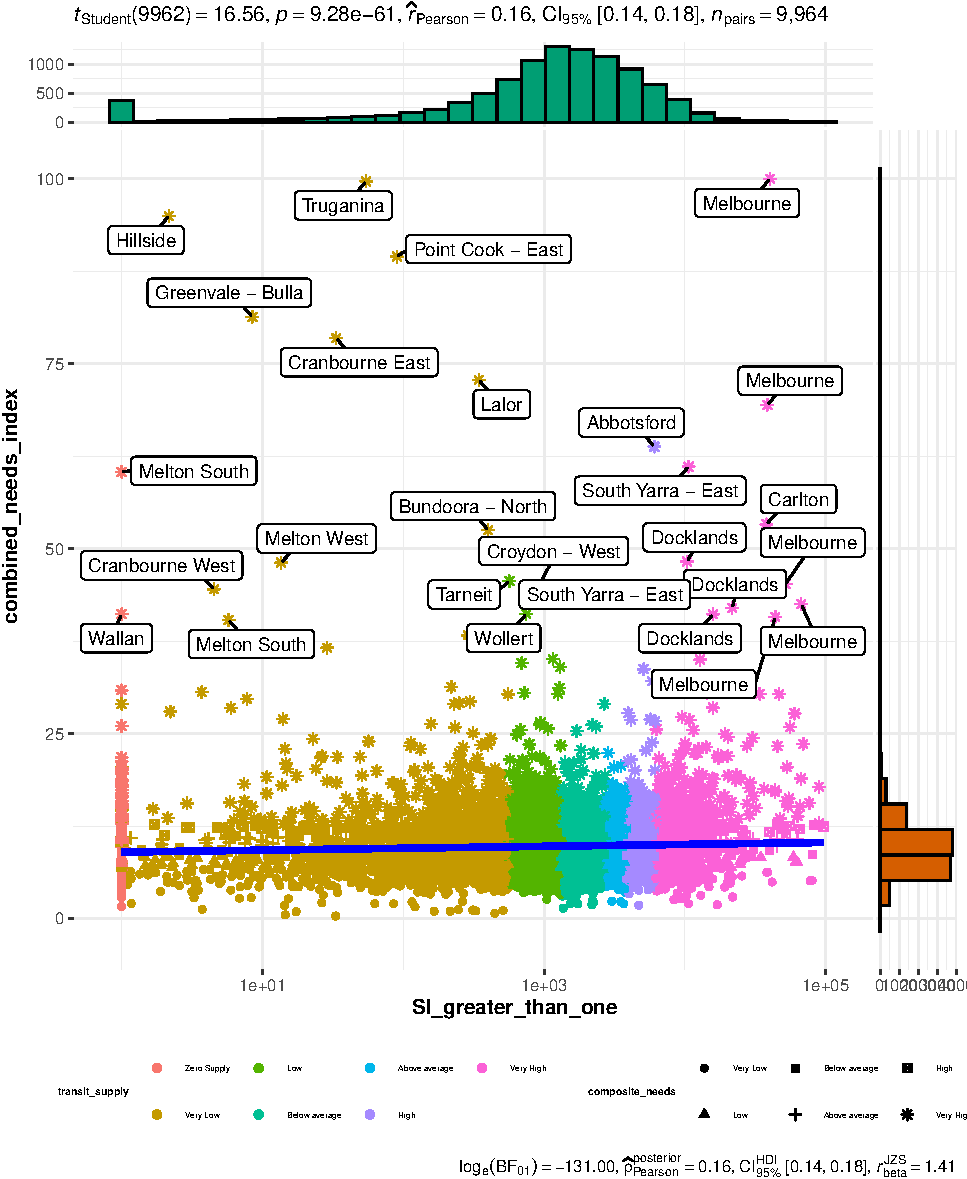
\includegraphics{Leveraging_GTFS_to_assess_transit_supply_Transport_Geography_files/figure-latex/Greater_Melbourne_2016_needs_gap-1.pdf}
\caption{Greater Melbourne 2016, SI and Combined Needs Index scores,
with SI scores \textless{} 1 rounded up to equal 1.}
\end{figure}

Figure \ref{fig:Greater_Melbourne_2016_needs_gap} compares SI and
Combined Needs Index scores for SA1s in 2016. There is a significant,
but only weakly positive relationship.

\begin{table}

\caption{\label{tab:Greater_Melbourne_2016_needs_gap_zones}Greater Melbourne 2016, SA1s within each SI and Combined Needs Index grouping}
\centering
\fontsize{7}{9}\selectfont
\begin{tabular}[t]{l|r|r|r|r|r|r|r}
\hline
transit\_supply & Very Low & Low & Below average & Above average & High & Very High & Total\\
\hline
Zero Supply & 4.8\%    (91) & 3.5\%    (66) & 2.5\%    (47) & 2.4\%    (34) & 2.0\%    (28) & 3.2\%    (46) & 3.1\%   (312)\\
\hline
Very Low & 26.1\%   (497) & 23.2\%   (442) & 20.9\%   (397) & 20.4\%   (290) & 19.8\%   (281) & 22.5\%   (319) & 22.3\% (2,226)\\
\hline
Low & 24.1\%   (458) & 24.5\%   (467) & 24.4\%   (464) & 22.3\%   (317) & 21.7\%   (308) & 19.7\%   (279) & 23.0\% (2,293)\\
\hline
Below average & 24.9\%   (473) & 24.5\%   (467) & 24.1\%   (459) & 23.8\%   (338) & 23.2\%   (329) & 17.6\%   (249) & 23.2\% (2,315)\\
\hline
Above average & 7.4\%   (140) & 9.2\%   (175) & 10.2\%   (194) & 10.5\%   (149) & 10.6\%   (150) & 9.2\%   (131) & 9.4\%   (939)\\
\hline
High & 6.5\%   (123) & 7.5\%   (142) & 10.7\%   (203) & 10.2\%   (145) & 12.0\%   (170) & 10.9\%   (155) & 9.4\%   (938)\\
\hline
Very High & 6.4\%   (121) & 7.6\%   (144) & 7.3\%   (139) & 10.3\%   (146) & 10.7\%   (152) & 16.9\%   (239) & 9.4\%   (941)\\
\hline
Total & 100.0\% (1,903) & 100.0\% (1,903) & 100.0\% (1,903) & 100.0\% (1,419) & 100.0\% (1,418) & 100.0\% (1,418) & 100.0\% (9,964)\\
\hline
\end{tabular}
\end{table}

\begin{figure}
\centering
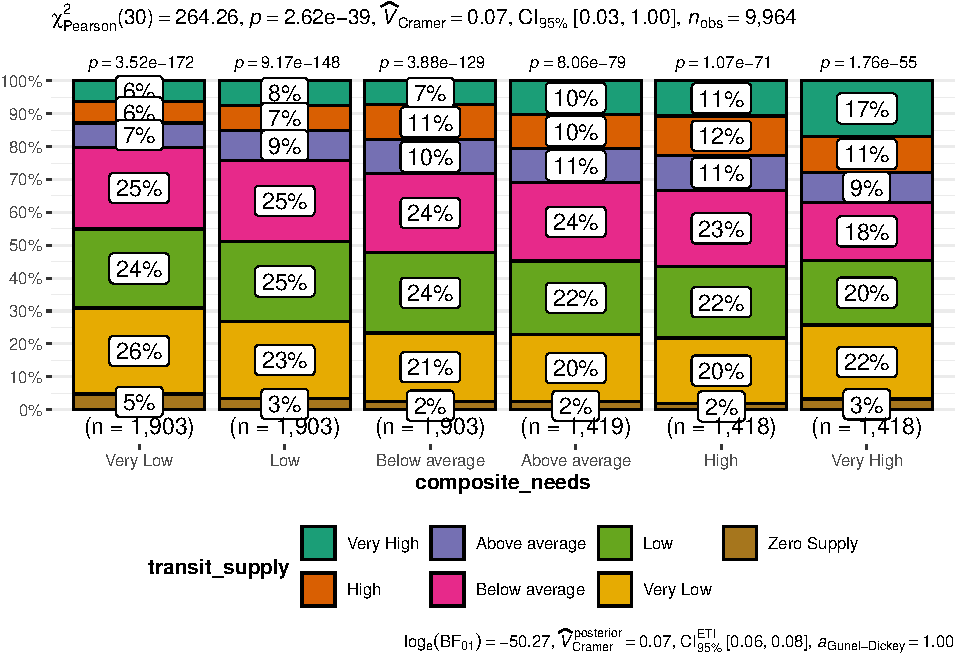
\includegraphics{Leveraging_GTFS_to_assess_transit_supply_Transport_Geography_files/figure-latex/Greater_Melbourne_2016_needs_gap_zones-1.pdf}
\caption{Greater Melbourne 2016, SA1s within each SI and Combined Needs
Index grouping}
\end{figure}

Figure \ref{fig:Greater_Melbourne_2016_needs_gap_zones} and Table
\ref{tab:Greater_Melbourne_2016_needs_gap_zones} compares the SI and
Combined Needs Index groupings for 2016. There is a statistically
significant relationship, although this appears to be weak. 365 SA1s
have zero or very low transit supply, but very high social needs. This
represents 3.7\% of the 9,964 SA1s within Greater Melbourne, and is a
higher proportion than that reported for 2006 (85 of 5,720 CCDs
(1.6\%)).

\begin{table}

\caption{\label{tab:Greater_Melbourne_2016_needs_gap_population}Greater Melbourne 2016, Population in each SI and Combined Needs Index grouping}
\centering
\fontsize{7}{9}\selectfont
\begin{tabular}[t]{l|r|r|r|r|r|r|r}
\hline
transit\_supply & Very Low & Low & Below average & Above average & High & Very High & Total\\
\hline
Zero Supply & 4.3\%  (22,012) & 3.3\%  (22,544) & 2.4\%  (18,784) & 2.3\%  (15,402) & 1.9\%  (14,790) & 3.6\%    (38,050) & 2.9\%   (131,582)\\
\hline
Very Low & 24.8\% (126,298) & 23.1\% (156,359) & 20.8\% (165,350) & 20.5\% (138,710) & 20.1\% (153,169) & 25.1\%   (263,693) & 22.4\% (1,003,579)\\
\hline
Low & 24.8\% (126,411) & 24.9\% (168,228) & 24.8\% (197,542) & 22.8\% (154,275) & 22.1\% (168,541) & 19.1\%   (200,937) & 22.7\% (1,015,934)\\
\hline
Below average & 25.4\% (129,440) & 25.1\% (169,849) & 24.4\% (193,915) & 24.1\% (163,593) & 23.2\% (177,044) & 15.7\%   (164,681) & 22.3\%   (998,522)\\
\hline
Above average & 7.5\%  (38,003) & 9.1\%  (61,679) & 10.1\%  (80,591) & 10.3\%  (70,066) & 10.5\%  (80,172) & 8.1\%    (84,562) & 9.3\%   (415,073)\\
\hline
High & 6.6\%  (33,334) & 7.3\%  (49,615) & 10.4\%  (83,055) & 9.9\%  (67,061) & 11.7\%  (89,517) & 10.1\%   (105,960) & 9.6\%   (428,542)\\
\hline
Very High & 6.6\%  (33,361) & 7.2\%  (48,441) & 7.1\%  (56,303) & 10.1\%  (68,467) & 10.4\%  (79,329) & 18.3\%   (192,038) & 10.7\%   (477,939)\\
\hline
Total & 100.0\% (508,859) & 100.0\% (676,715) & 100.0\% (795,540) & 100.0\% (677,574) & 100.0\% (762,562) & 100.0\% (1,049,921) & 100.0\% (4,471,171)\\
\hline
\end{tabular}
\end{table}

\begin{figure}
\centering
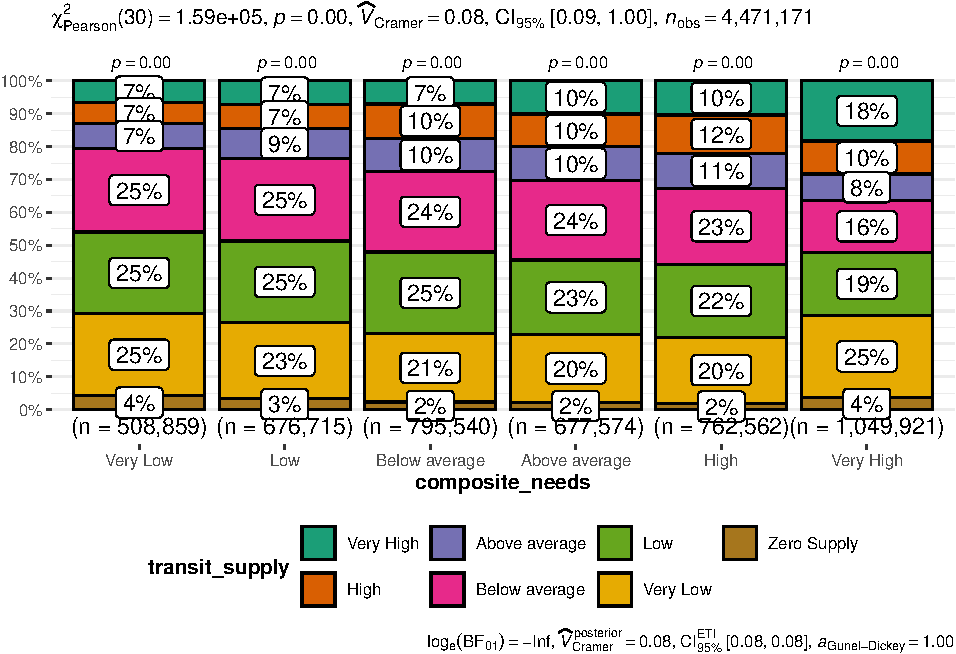
\includegraphics{Leveraging_GTFS_to_assess_transit_supply_Transport_Geography_files/figure-latex/Greater_Melbourne_2016_needs_gap_population-1.pdf}
\caption{Greater Melbourne 2016, Populations within each SI and Combined
Needs Index grouping}
\end{figure}

Figure \ref{fig:Greater_Melbourne_2016_needs_gap_population} and Table
\ref{tab:Greater_Melbourne_2016_needs_gap_population} compares the
populations within each SI and Combined Needs Index grouping for 2016.
There is a statistically significant relationship, although this appears
to be weak. \ensuremath{3.01743\times 10^{5}} people live within SA1s
that have zero or very low transit supply, but very high social needs.
This represents 6.7\% of the 4,471,171 people within Greater Melbourne,
and is a lower proportion than that reported for 2006 (37,699 of 3.3
million people (8.2\%)).

\begin{figure}
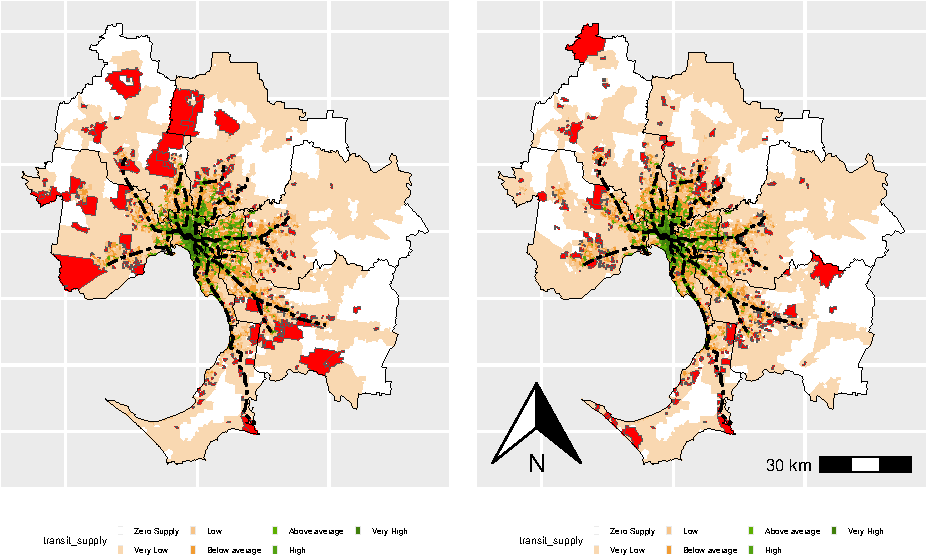
\includegraphics[width=1\linewidth]{Leveraging_GTFS_to_assess_transit_supply_Transport_Geography_files/figure-latex/Greater_Melbourne_2016_needs_gap_map-1} \caption{Greater Melbourne 2016 SI groupings, overlayed with SA1s with very high transport need areas with zero or very low public transport supply (red).}\label{fig:Greater_Melbourne_2016_needs_gap_map}
\end{figure}

Figure \ref{fig:Greater_Melbourne_2016_needs_gap_map} shows SA1 zones in
Greater Melbourne with Very High transport needs, but Very Low or Zero
transit supply for 2016 (left) and 2021 (right) in red. There are no
SA1s within the inner suburbs with Very High transport needs, but Very
Low or Zero transit supply in either 2016 or 2021. In the middle suburbs
there appear to be some minor shifts, but the overall pattern in both
2016 and 2021 appears to be that there are isolated areas of Very High
transport needs, but Very Low or Zero transit supply in between train
lines. In the outer suburbs, however:

\begin{itemize}
\tightlist
\item
  areas around Werribee (south-west) continue to have Very High
  transport needs, but Very Low or Zero transit supply, and many of the
  changes between 2016 and 2021 appear to be related to new SA1 zones
  being added.
\item
  there appears to have been some improvement around Bacchus Marsh and
  Melton (west), but again, this may be an aterfact of some of the 2016
  SA1 zones having been split in 2021.\\
\item
  no improvements around Gisbourne (west-north-west)
\item
  some shifts around Lancefield and Romsey (north-west), Kilmore and
  west of Craigieburn (north-north-west), but again these may being in
  part due to boundary changes;
\item
  no improvement around Mernda, Diamond Creek and (west of) Hurstbridge
  (north-east) or around the outer eastern or south-eastern suburbs;
\item
  additions in the outter east and south including in parts of the
  Mornington Peninsula (south) and places close to Emerald and Gembrook.
\end{itemize}

\section{Discussion}\label{discussion}

\subsection{Limitations}\label{limitations}

\subsection{Directions for furture
research}\label{directions-for-furture-research}

\section{Conclusions}\label{conclusions}

\section*{References}\label{references}
\addcontentsline{toc}{section}{References}

\section{Appendix A - GCCSA maps by
SA1}\label{appendix-a---gccsa-maps-by-sa1}

\renewcommand\refname{Holding for spare stuff}
\bibliography{References.bib, packages.bib}


\end{document}
